\chapter{Principal component analysis}
\label{ch:pca}

\begin{learningobjectives}
After this chapter, you should be able to:
\begin{itemize}
  \item derive principal directions from the covariance Rayleigh quotient;
  \item connect covariance eigendecomposition, singular values, scores, loadings,
  explained variance, and low-rank reconstruction;
  \item explain centering, scaling, whitening, sign ambiguity, and rank choice;
  \item place PCA inside a leakage-safe supervised pipeline; and
  \item evaluate predictive quality and computational cost as separate outcomes.
\end{itemize}
\end{learningobjectives}

\begin{chapterconnection}
Chapter~\ref{ch:unsupervised-learning} showed that dimensionality reduction must
name what it preserves. PCA preserves as much sample variance as possible among
linear orthogonal projections, equivalently minimizing squared low-rank
reconstruction error. This chapter develops that statement as a theorem and
then tests whether the representation helps a supervised digit classifier.
\end{chapterconnection}

\section{From many measurements to fewer coordinates}

Let $X\in\mathbb{R}^{n\times p}$ contain observations as rows and numerical
features as columns. Define the feature mean $\bar x$ and centered matrix
\[
X_c=X-\mathbf{1}\bar x^\top.
\]
A unit vector $v\in\mathbb{R}^p$ defines one coordinate per observation:
$z=X_cv$. The sample variance of these scores is
\begin{equation}
\label{eq:pca-rayleigh}
\frac{1}{n-1}\lVert X_cv\rVert_2^2
=v^\top\left(\frac{X_c^\top X_c}{n-1}\right)v
=v^\top S v,
\end{equation}
where $S$ is the sample covariance matrix.

PCA chooses the unit direction that maximizes Equation~\eqref{eq:pca-rayleigh},
then chooses later directions under orthogonality constraints. Loadings describe
directions in feature space; scores describe observations in component space.
Confusing the two is a common source of incorrect interpretation.

\begin{theorem}[the first principal direction]
\label{thm:first-pc}
Let $S$ be a symmetric positive-semidefinite covariance matrix with largest
eigenvalue $\lambda_1$. Then
\[
\max_{\lVert v\rVert_2=1}v^\top S v=\lambda_1,
\]
and every unit eigenvector associated with $\lambda_1$ is a maximizer.
\end{theorem}

\begin{proof}
The spectral theorem gives an orthonormal eigenbasis $q_1,\ldots,q_p$ with
eigenvalues $\lambda_1\ge\cdots\ge\lambda_p\ge0$. Write
$v=\sum_j a_jq_j$ with $\sum_j a_j^2=1$. Then
\[
v^\top Sv=\sum_{j=1}^p\lambda_j a_j^2
\le\lambda_1\sum_{j=1}^p a_j^2=\lambda_1.
\]
Equality is attained by $v=q_1$, and by any unit vector in the top eigenspace
when the largest eigenvalue is repeated.
\end{proof}

The proof clarifies nonuniqueness. If the largest eigenvalue is repeated, there
is no unique first axis inside that eigenspace. Even for a simple eigenvalue,
$v$ and $-v$ are the same axis. Software may return opposite signs without
disagreement.

\section{Projection and reconstruction}

Collect the first $k$ orthonormal loading vectors as columns of
$V_k\in\mathbb{R}^{p\times k}$. Component scores and centered reconstruction are
\[
Z=X_cV_k,
\qquad
\widehat X_c=ZV_k^\top=X_cV_kV_k^\top.
\]
The matrix $V_kV_k^\top$ is the orthogonal projector onto the retained
subspace. Each reconstruction residual is perpendicular to that subspace.

\begin{center}
  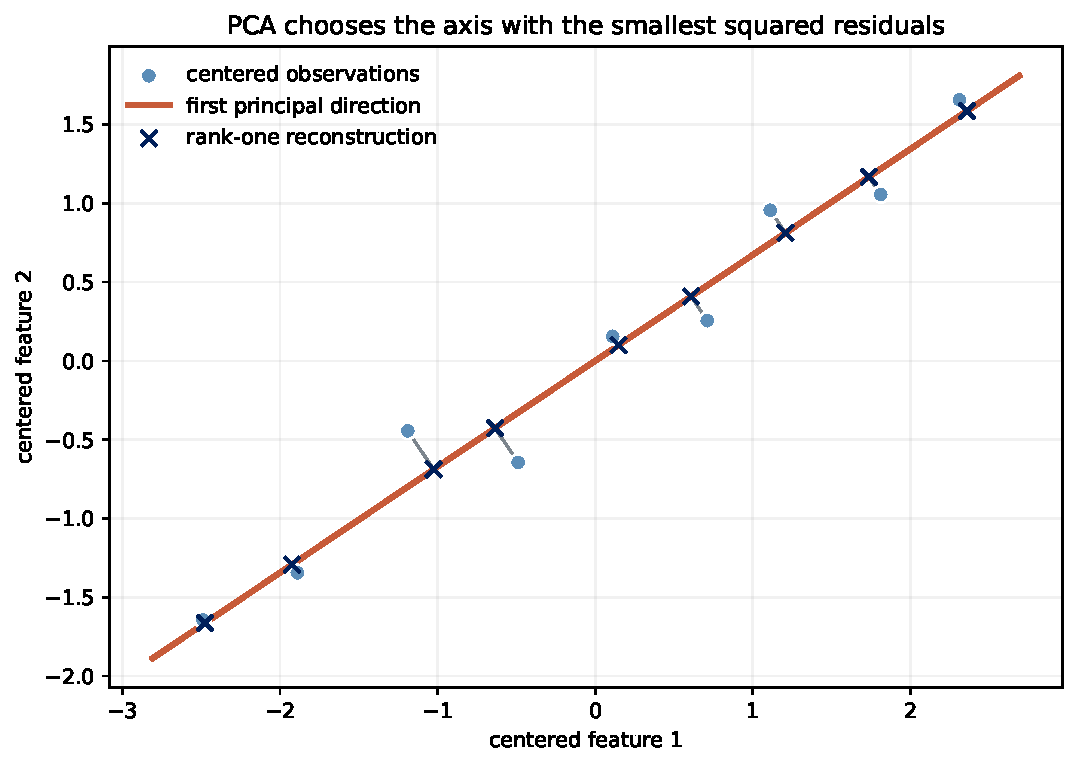
\includegraphics[width=0.82\textwidth]{figures/generated/pca-projection-geometry.pdf}
\end{center}

\begin{theorem}[PCA minimizes squared rank-$k$ reconstruction]
\label{thm:pca-reconstruction}
If $X_c=U\Sigma V^\top$ is a singular value decomposition with
$\sigma_1\ge\cdots\ge0$, then
\[
X_{c,k}=U_k\Sigma_kV_k^\top=X_cV_kV_k^\top
\]
minimizes $\lVert X_c-B\rVert_F$ over matrices $B$ of rank at most $k$, and
\[
\lVert X_c-X_{c,k}\rVert_F^2=\sum_{j>k}\sigma_j^2.
\]
\end{theorem}

\begin{proof}[Proof sketch]
Orthogonal transformations preserve the Frobenius norm. In singular-vector
coordinates, approximating $X_c$ is equivalent to approximating the diagonal
matrix $\Sigma$. A rank-$k$ matrix can preserve at most $k$ independent singular
directions. Retaining the $k$ largest diagonal values leaves squared error
$\sum_{j>k}\sigma_j^2$; replacing any retained singular value by a smaller
discarded one cannot reduce this error. This is the Eckart--Young--Mirsky
theorem specialized to the Frobenius norm.
\end{proof}

The covariance eigenvalues and singular values obey
\[
\lambda_j=\frac{\sigma_j^2}{n-1}.
\]
Thus maximum retained variance and minimum squared reconstruction are the same
linear subspace problem.

\section{Explained variance is descriptive, not predictive}

The explained-variance ratio of component $j$ is
\[
r_j=\frac{\lambda_j}{\sum_{\ell=1}^{p}\lambda_\ell},
\]
and $\sum_{j=1}^k r_j$ is the fraction of total sample variance retained by the
first $k$ components. A scree plot displays $r_j$; a cumulative plot displays
their partial sums.

A 90\% or 95\% threshold is a policy, not a law. It optimizes neither class
accuracy nor scientific relevance. A rare disease signal, weak spectral line,
or safety-critical failure can occupy a low-variance direction. Conversely,
high variance can represent illumination, batch, site, or instrument effects.

\begin{misconceptionbox}
\textbf{Misconception:} retaining 95\% variance retains 95\% of the information.
\textbf{Correction:} variance is a particular second-moment summary under the
chosen coordinates and scaling. ``Information'' requires a task or probabilistic
definition. PCA may discard a low-variance direction that perfectly separates a
target.
\end{misconceptionbox}

\conceptcheck{Construct two features for which the lower-variance feature
perfectly predicts a binary target while the higher-variance feature is pure
noise. What will one-component PCA prefer?}

\section{Centering, scaling, and whitening}

Centering is part of ordinary PCA because the component subspace describes
variation around the mean. Without centering, the origin becomes part of the
model and the leading direction can mostly describe the mean offset.

Scaling is separate. Covariance PCA respects original numerical units;
correlation PCA first standardizes features. Standardization is often useful
when units are arbitrary or incomparable, but can amplify measurement noise in
nearly constant features. Domain knowledge should decide whether a one-unit, a
one-standard-deviation, or an uncertainty-weighted change is comparable.

Whitening rescales retained scores so their sample variances are one. It can
serve downstream methods whose assumptions favor spherical coordinates, but it
throws away the component variance magnitudes and may magnify weak directions.
The words \emph{PCA} and \emph{whitening} are not synonyms.

Fitted means, scales, loadings, and optional whitening factors belong to the
artifact. New observations use those training values; they do not recompute
them from a prediction batch.

\section{Computation through the singular value decomposition}

Directly forming $S=X_c^\top X_c/(n-1)$ squares the condition number and can be
wasteful. Numerical software typically computes an SVD of the centered matrix
or uses an equivalent solver selected for matrix shape and requested rank.

A dense full SVD costs roughly
$O(\min\{np^2,n^2p\})$ operations and stores the data and factors. Randomized
methods can estimate a leading subspace when $k\ll\min(n,p)$. Incremental PCA
updates a bounded representation across batches when the complete matrix does
not fit memory. Truncated SVD can preserve sparsity because it need not center,
but that makes its semantics different from centered PCA.

The course implementation uses full SVD so every mathematical state is visible.
It applies a deterministic sign convention for stable displays: within each
component, the loading with greatest absolute value is made positive. This does
not change scores up to corresponding sign or change the subspace.

\begin{professionalbox}
Test subspaces and reconstructions, not exact loading signs alone. Useful
properties include orthonormal components, centered training scores, decreasing
reconstruction error as rank grows, full-rank recovery, shape validation, and
failure before fitting.
\end{professionalbox}

\section{Worked example: real handwritten digits}

The course database stores 1,797 real handwritten digits, each represented by
64 grayscale intensities from an $8\times8$ image. The split occurs before PCA.
The training mean and directions are then applied unchanged to held-out images.

The reconstruction gallery below is not merely decorative. At rank two, broad
intensity structure remains but digit identity is often ambiguous. Higher ranks
restore strokes and local variation. Reconstruction error must decrease as rank
increases, but a visually recognizable reconstruction does not guarantee a
better classifier.

\begin{center}
  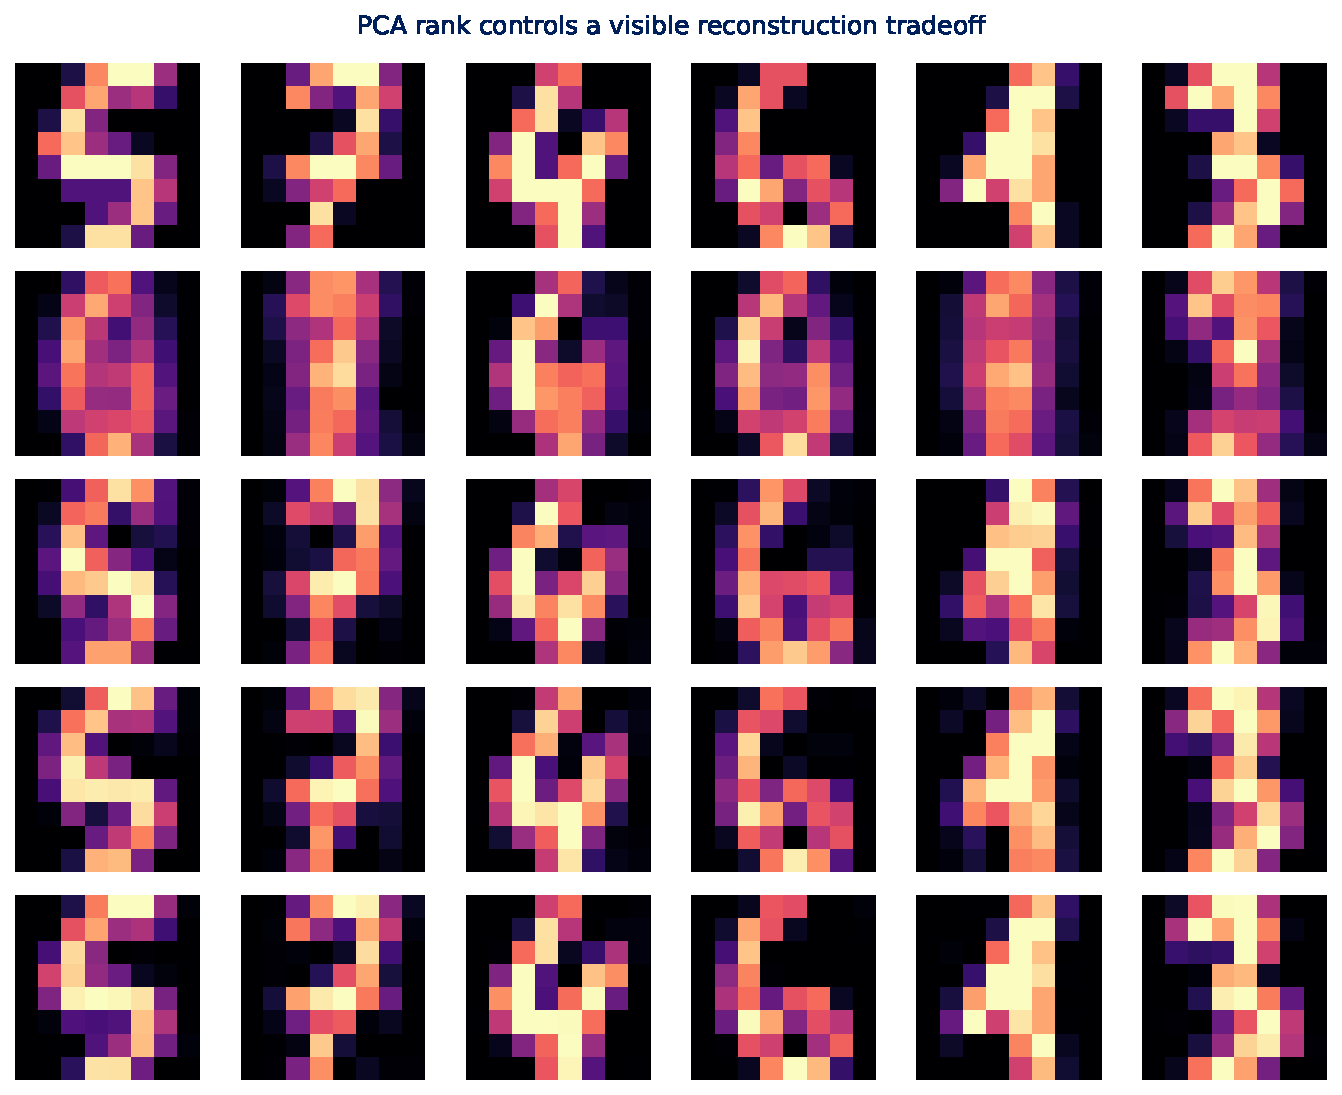
\includegraphics[width=0.88\textwidth]{figures/generated/pca-digits-reconstruction.pdf}
\end{center}

PCA loadings can be reshaped into ``eigendigits.'' Positive and negative pixels
show how a component changes an image relative to the training mean. A loading
is a direction, not a prototypical digit, and its sign is arbitrary.

\section{PCA as part of a supervised system}

To use PCA with $k$-nearest-neighbor classification, define one pipeline:
\[
x\longmapsto \text{training-fitted scale}
\longmapsto \text{training-fitted PCA}
\longmapsto \text{KNN prediction}.
\]
During cross-validation, every fold must refit both transformations using only
its training portion. Fitting PCA once on all observations before folds leaks
validation information through means and directions even though PCA never sees
the target.

The real digit experiment below compares the number of coordinates used in each
distance with held-out accuracy. Thirty PCA coordinates use less than half the
coordinate operations of 64-pixel KNN while producing very similar accuracy in
this split. The notebook additionally times the complete prediction pipeline,
including PCA transformation, using warmed repeated measurements.

\begin{center}
  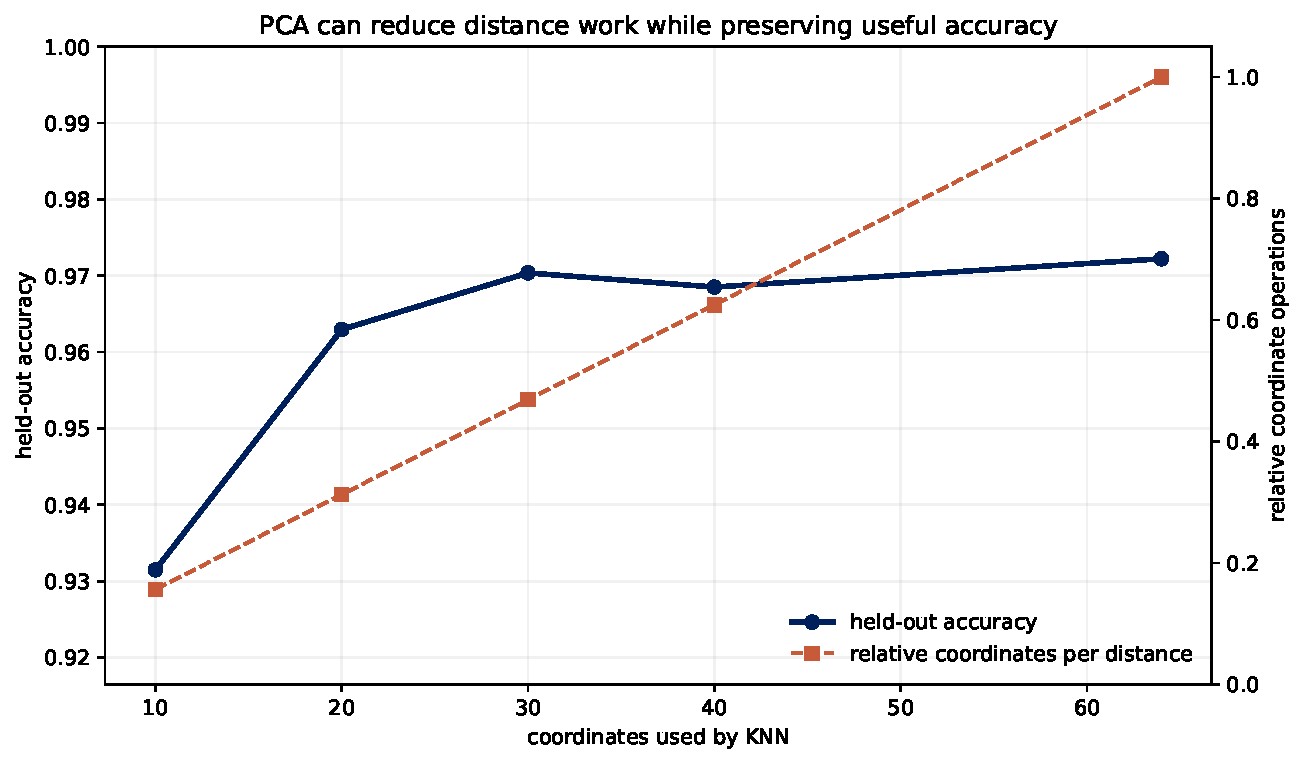
\includegraphics[width=0.88\textwidth]{figures/generated/pca-supervised-tradeoff.pdf}
\end{center}

This is a real performance gain when the operational objective values lower
prediction cost at comparable accuracy. It is not proof that PCA always speeds
KNN: transform overhead, optimized kernels, memory layout, training size,
hardware, batch size, and retained rank all matter. PCA also has training cost.

\begin{workedexample}{a promotion decision with two axes}
A digit-retrieval service compares scaled 64-coordinate KNN with a 30-component
PCA pipeline. Training-only cross-validation chooses the candidate rank. On a
locked test set, accuracy changes from $0.972$ to $0.970$, while one local
benchmark reduces batch prediction time from roughly $81$ ms to $3$ ms. Repeated
measurements on the target host confirm the direction of the latency change.

The team does not report ``PCA improved the model.'' It reports a candidate
that traded an estimated $0.2$ percentage points of accuracy for substantially
lower measured inference cost under a named environment. Whether to promote it
depends on accuracy tolerance, latency objective, traffic, artifact behavior,
and uncertainty. The exact timing is not generalized beyond that environment.
\end{workedexample}

\section{When PCA is the wrong representation}

PCA is linear, global, variance-driven, and based on squared Euclidean
reconstruction. It can fail when the useful structure is curved, categorical,
sparse, robust rather than least-squares, local rather than global, or tied to a
target in low variance directions. Kernel PCA supplies nonlinear features but
introduces kernel and scaling choices and typically poor out-of-sample and
large-$n$ scaling. Neighborhood methods such as t-SNE and UMAP are valuable for
visualization but require their own objective-specific interpretation; apparent
cluster sizes and global distances can be misleading.

Supervised alternatives such as partial least squares or learned neural
representations use targets or task losses. They may better serve prediction,
but answer a different question and require supervised evaluation.

\section{Engineering and monitoring the representation}

A PCA artifact contains input feature order, units, missing-value policy,
training mean, optional scales, components, singular values, retained-rank
rule, solver, data and code provenance, and compatibility version. Prediction
must reject missing, reordered, nonfinite, or incompatible features rather than
silently project them.

Monitor upstream schema and missingness, score distributions, reconstruction
error, and downstream performance when outcomes arrive. Component sign flips
or rotations within a repeated-eigenvalue subspace can change coordinates
without changing the represented subspace. Monitoring should therefore include
subspace-aware quantities and task evidence rather than brittle equality of
individual loadings.

\section{Exercises}
\begin{enumerate}
  \item \textbf{Derivation.} Use Lagrange multipliers on
  Equation~\eqref{eq:pca-rayleigh} and recover the covariance eigenvalue equation.
  Explain what the argument alone does not prove about a global maximum.
  \item \textbf{Projection.} Prove that $V_kV_k^\top$ is symmetric and idempotent
  when $V_k^\top V_k=I$. Conclude that it is an orthogonal projector.
  \item \textbf{Error.} Starting from Theorem~\ref{thm:pca-reconstruction}, show
  that the average per-observation squared residual equals
  $\sum_{j>k}\sigma_j^2/n$.
  \item \textbf{Counterexample.} Construct a labeled dataset in which the
  highest-variance direction is independent of the target and the
  lowest-variance direction separates it perfectly.
  \item \textbf{Pipeline.} Draw a nested cross-validation design that chooses
  scaling, PCA rank, KNN neighbor count, and distance weighting. Mark every fit
  boundary and final untouched estimate.
  \item \textbf{Performance.} Benchmark prediction latency across batch sizes.
  Report warm-up, repetitions, median and spread, environment identity, accuracy,
  retained rank, and whether PCA transform time is included.
  \item \textbf{Contribution.} Add one reviewed capability to a PCA implementation:
  a variance threshold, randomized solver, or incremental batches. Supply a
  NumPy-style public contract, analytic property tests, invalid-input tests,
  trusted-library comparison, real-data notebook, and PR discussion of numerical
  limitations.
\end{enumerate}

\begin{chapterreview}
PCA centers observations and selects orthogonal directions of decreasing
variance. Covariance eigenvectors and right singular vectors describe the same
principal subspace; truncated SVD gives the optimal linear rank-$k$ squared
reconstruction. Scores locate observations, loadings define directions, signs
are arbitrary, and scaling changes the question. Explained variance is not
target relevance. In supervised use, PCA belongs inside every split and must be
evaluated jointly for predictive, computational, and operational behavior.
\end{chapterreview}

\begin{notebooklink}
Lecture 16 notebook 01 derives PCA, visualizes scores, loadings, and real digit
reconstructions, exercises the tested \texttt{PrincipalComponentProjector}, and
benchmarks a leakage-safe PCA--KNN pipeline for accuracy and prediction cost.
\end{notebooklink}
